\documentclass{article}

% set font encoding for PDFLaTeX or XeLaTeX
\usepackage{ifxetex}
\ifxetex
  \usepackage{fontspec}
\else
  \usepackage[T1]{fontenc}
  \usepackage[utf8]{inputenc}
  \usepackage{lmodern}
  \usepackage{graphicx}
\fi

% used in maketitle
\title{
        \begin{center}
        
\includegraphics[width=8cm]{Unison.png}
        \end{center}
        \newline
       Reporte de Actividad 1}
\author{Jose "Buma" Burruel Martinez}
\date{30 de Enero del 2018}

% Enable SageTeX to run SageMath code right inside this LaTeX file.
% documentation: http://mirrors.ctan.org/macros/latex/contrib/sagetex/sagetexpackage.pdf
% \usepackage{sagetex}


\begin{document}


\maketitle {Atmósfera de la Tierra}

\newpage
\section{Síntesis}

\subsection{Introducción}
La atmosfera de la tierra es una capa de gases, comúnmente conocida como Aire, que rodea al planeta Tierra y es retenida por la gravedad de la misma. La atmósfera protege la vida en la tierra creando pressión que permite la existencia de agua líquida, absorbiendo los rayos ultravioleta de la radiacion solar, calentando la superficie con el efecto invernadero y reduciendo las temperaturas extremas del día y la noche.


Al estudio de la atmósfera de la Tierra y sus procesos se le llama Ciencia Atmosférica (o Aerología).

\subsection{Composición}
En volumen, el aire seco contiene 78.09\% nitrógeno, 20.95\% oxígeno, 0.93\% argón, 0.04\% dióxido de carbono, y otras pequeñas cantidades de otros gases. Además,el aire también contiene una cantidad variable de vapor de agua, en promedio alrededor de 1\% al nivel del mar, y 0.4\% en el resto de la atmósfera. Esta composición de gases  varía con respecto a la región y localidad de donde se haga el estudio de la misma.

\begin{figure}
    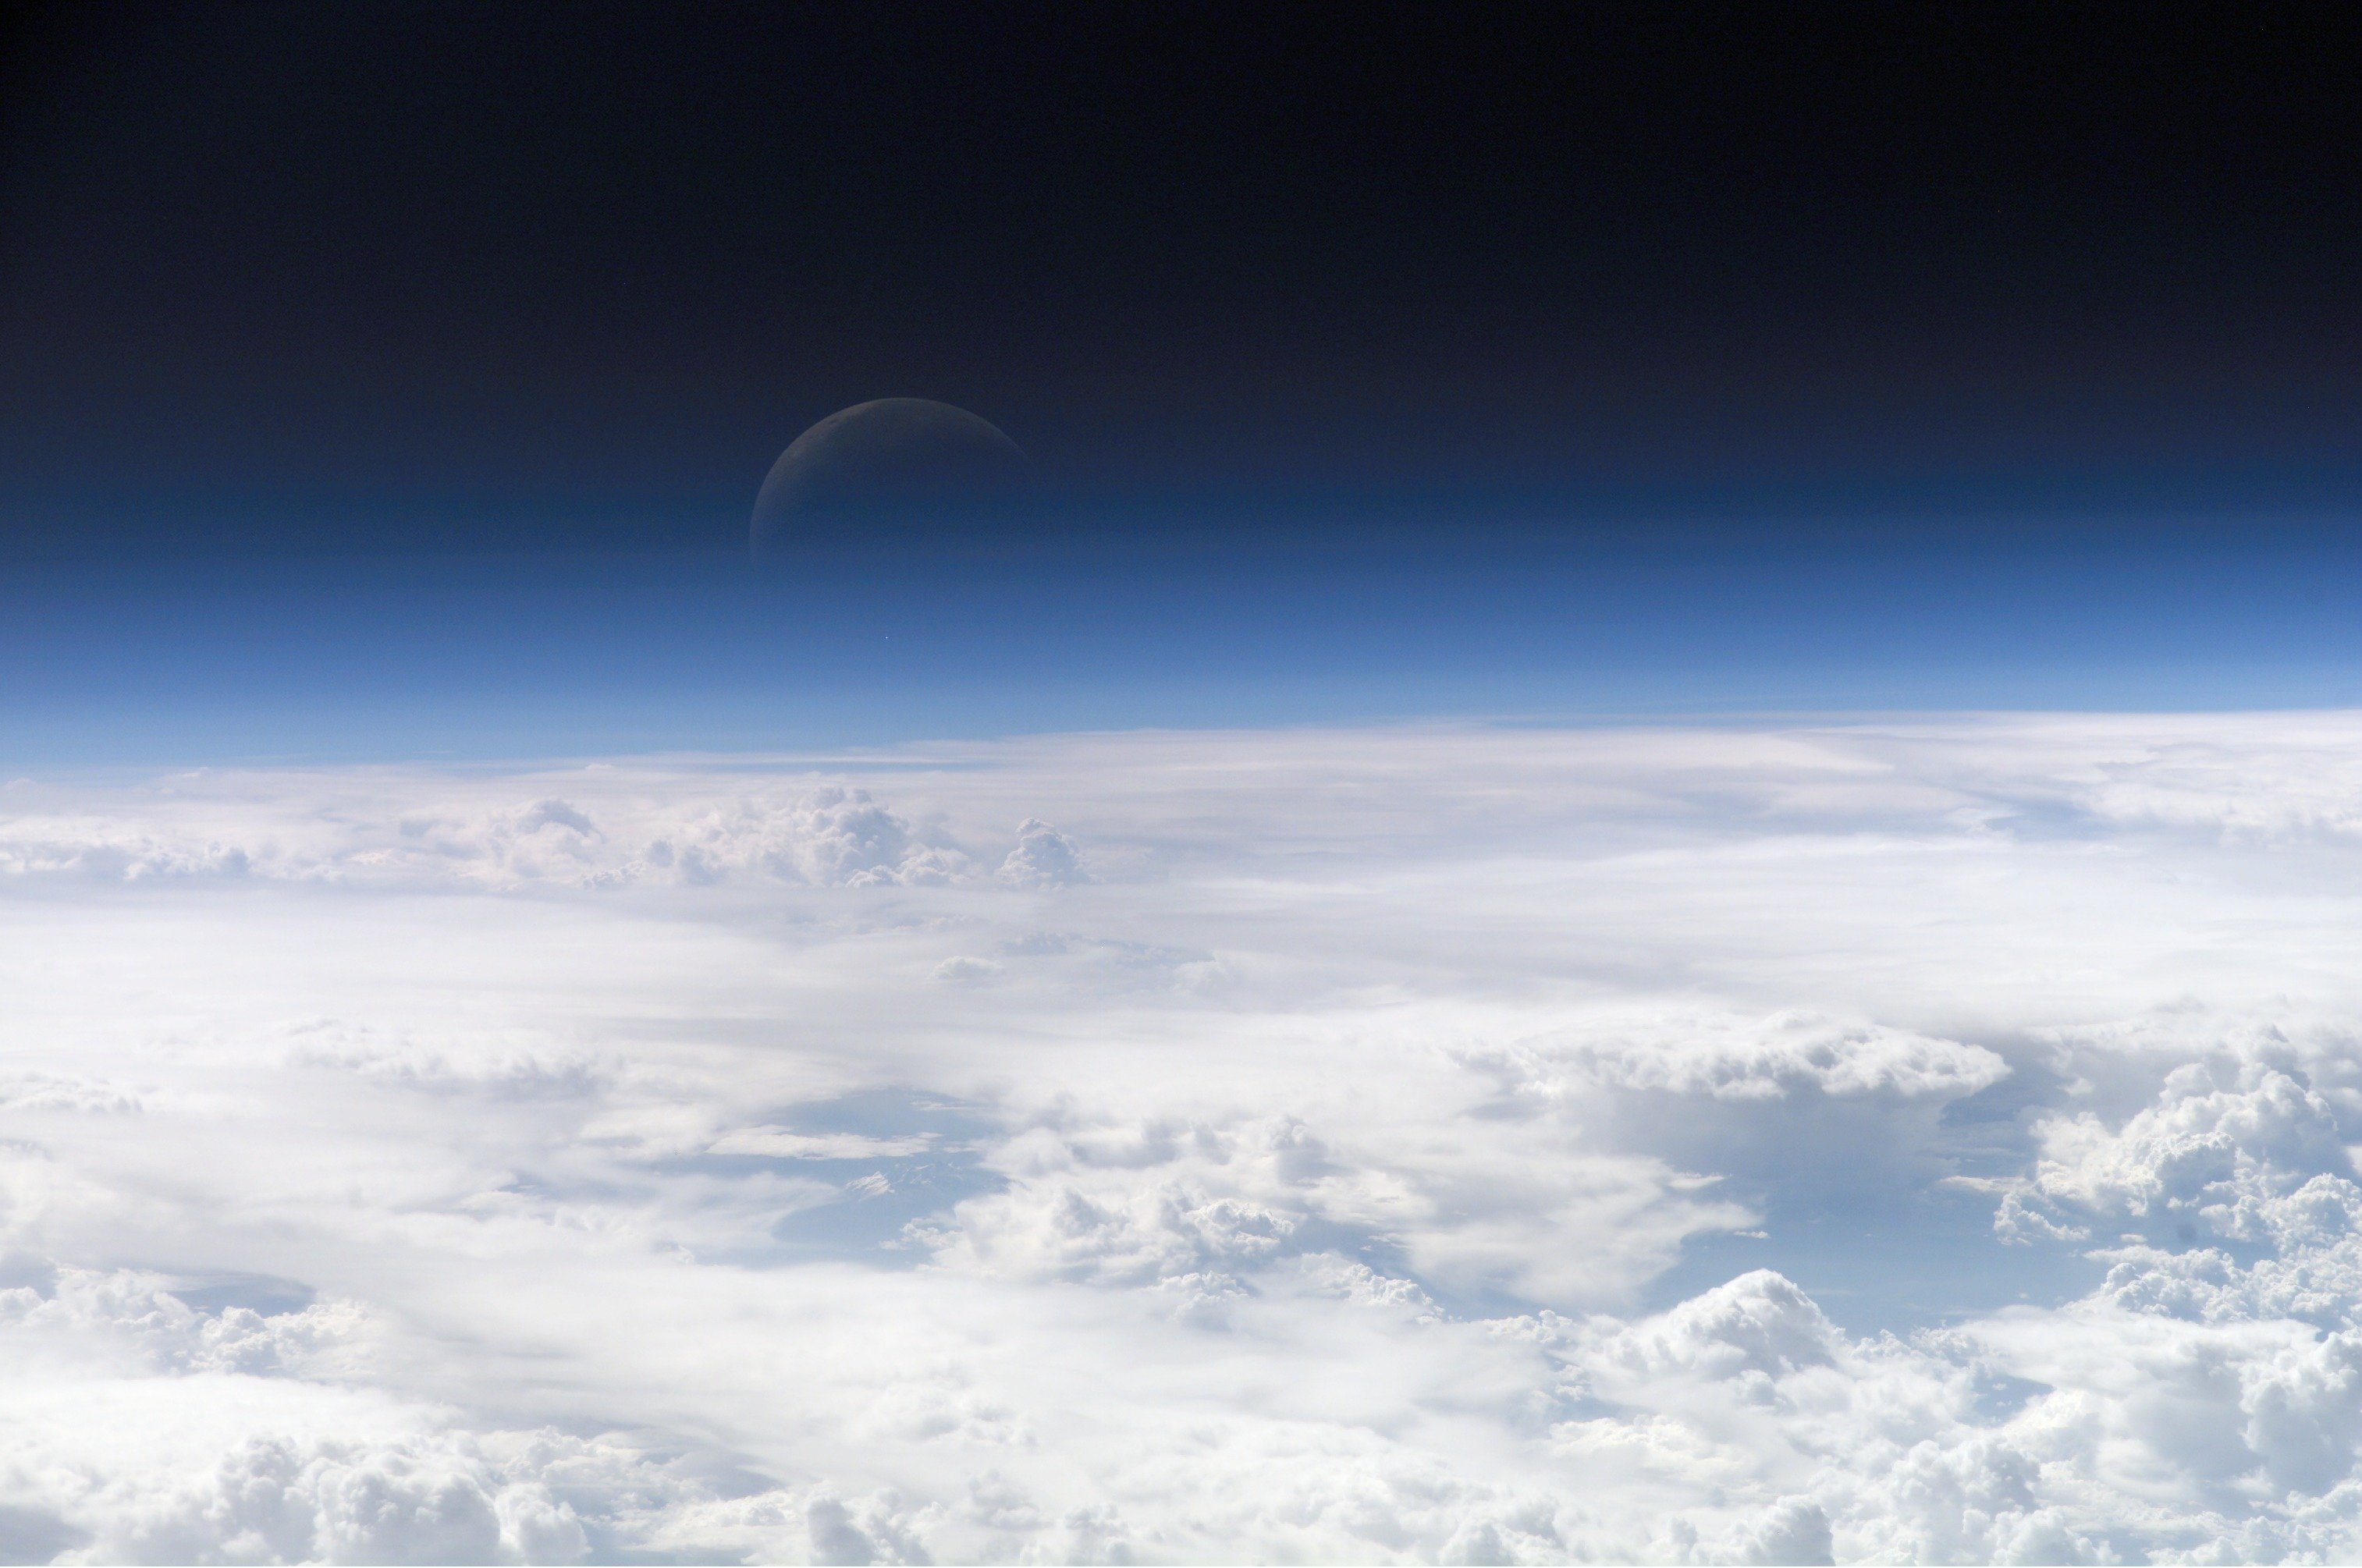
\includegraphics[width=\linewidth]{Top_of_Atmosphere.jpg}
    \caption{Vista aerea de la atmósfera. By NASA}
    \label{fig:foto1}
\end{figure}
    


\subsection{Estructura de la atmósfera}
En general, la presión del aire y la densidad del mismo decrece con la altura de la atmósfera. Debido a que el patrón general de temperatura/altitud es constante y medible por medios de instrumentación, el comportamiento de la temperatura permite dividir a la atmósfera en 5 capas principales:

\subsubsection{Exósfera}
Es la capa más lejana de la atmósfera de la tierra. Se extiende desde una altura de 700km arriba del nivel del mar, hasta 10'000km donde se combina con el viento solar.

Está constituída de extremadamente bajas densidades de hidrógeno, helio y otras varias moleculas pesadas que incluyen nitrógeno, oxígeno y dióxido de carbono en sus niveles más bajos.

\subsubsection{Termósfera}
La termósfera es la segunda más alta capa de la atmósfera terrestre. Se extiende sede una altitud de 80 km hasta un rango de 500-1000km, Lma temperatura de la termósfera se incrementa conforme la altura. diferente a la estratósfera debajo de ella, donde ocurre una inversión termal devido a la absorción de la radiación por el ozono. La temperatura de esta capa puede incrementarse hasta 1500C, sin embargo la baja densidad evita el contacto de estas moléculas tan calientes con algún otro objeto.

Esta capa está completamente libre de nubes y vapor de agua. Sin embargo, fenómenos no hidrometeorológicos ocurren en esta capa, como lo es la aurora boreal. La estación espacial internacional orbita ésta capa entre 350km y 430 km.

\subsubsection{Mesósfera}
Esta capa es la 3ra de la atmósfera, extendiendose desde una altitud desde 50km hasta 80km de altura.
En la mesósfera es donde los meteoros se desintegran en la entrada atmosférica. Es demasiado alta para permitir que un vehículo accese a ella, pero muy baja para que permitir una orbita de un cohete.

\subsubsection{Estratósfera}
Es la segunda más baja capa de la atmósfera de la Tierra. Se extiende desde unos 12km aproximadamente hasta los 50 km de altitud.

La presión atmosférica al punto más alto de la estratósfera es aproximadamente 1/1000 a la presión a nivel del mar. Ésta contiene a la capa de Ozono. La temperatura de la estratósfera incrementa conforme aumenta la altitud, debido a la absorción de los rayos ultravioleta por la capa de ozono, donde en el punto mas bajo puede ser de -60 Centígrados y en el punto más alto unos 0 grados Celisius.

\subsubsection{Troposfera}
La tropósfera es la capa más baja de la atmósfera terrestre. Se extiende desde el nivel del mar hasta alrededor de 12 km. Donde la temperatura decrece conforma la altura aumenta debido a la radiación que rebota de la superficie terrestre.
Casi todo el vapor de agua atmosférico o humedad se encuentra en la tropósfera, por lo tanto es la capa donde ocurre la mayoría del clima de la Tierra. Básicamente contiene todas las nubes asociadas climáticamente con el tiempo generado por activa circulación de aire, temperaturas locales, etc.

\subsection{Propiedades Físicas}

\subsubsection{Presión y grosor}
El promedio de presión atmosférica a nivel del mar está definido por el estandar internacional atmosférico como 101325 Pascales. La masa total atmosférica es de 5.1480x10$^18$.
en general, la masa de la atmósfera terrestre está distribuida aproximadamente de la siguiente manera:
\begin{itemize}
    \item 50\% está debajo de 5.6 km
    \item 90 está debajo de 16km
    \item 99.99997\% está debajo de 100km, en la linea Kérmán, que marca donde inicia el espacio.
 \end{itemize}
Ésta distribución de la masa atmosférica es lo que causa la presión, y siendo esta última la que genera los cambios climáticos.

\subsubsection{Temperatura y velocidad del sonido}
La temperatura tiene varias variaciones a diferentes alturas de la atmósfera. Aquí se enlista una vista bastante general:
\begin{itemize}
    \item La temperatura decrece con la altitud empezando por el nivel del mar.
    \item Al rededor de los 11km, la temperatura se estabiliza hasta el resto de la tropósfera.
    \item En la estratósfera y ionósfera, la temperatura aumenta conforme aumenta la altitud.
\end{itemize}
Debido a que en un gas ideal de constante composición, la velocidad del sonido depende solamente de la temperatura y no de la presión o densidad, ésta varía de la misma forma en la que cambia la temperatura.

\subsubsection{Densidad y masa}
El promedio de masa de la atmósfera es de 5x10$^15$ toneladas con variaciones de 1.2 o 1.5x10$^15$kg debido a cambios en el vapor de agua de la atmósfera dependiendo de si datos de vapor de agua y presión en la superficie son utilizados, esto de acuerdo al Centro Nacional Americano de Investigación Atmosférica.

La densidad del aire al nivel del mar es de 1.2 kg/m$^3$. Aunque la densidad no es medida directamente, si no que es calculada con medidas de temperatura, presión y humedad, utilizando ecuaciones de estado de aire (Que es una ley de Gas Ideal).





\newpage
\begin{figure}
    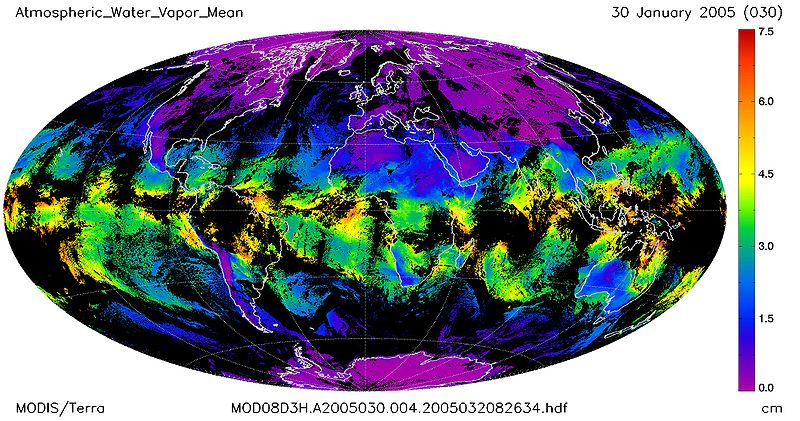
\includegraphics[width=\linewidth]{vapor.jpg}
    \caption{Gráfica de vapor de agua en la atmósfera. by NASA}
    \label{fig:foto2}
\end{figure}
\newpage

\subsection{Propiedades ópticas}
La radiación solar es la energía que la Tierra recibe del Sol. La Tierra también emite radiación de regreso al espacio pero en ondas más largas que no son visibles, y parte de la radiación recibida y emitida es absorbida o reflejada por la atmósfera.

\subsubsection{Dispersión}
Cuando la luz pasa por la atmósfera terrestre, los fotones interactúan con ella por Dispersión. Si la luz no interactúa con la atmósfera, se le llama Radiación directa, que es lo que pasa cuando vez diréctamente al Sol. Pero si sí interactúa con ella, se le llama Radiación indirecta.
Un ejemplo de eso último es el fenómeno llamado Dispersión de Rayleigh, donde las longitudes de onda más cortas (Azules) se dispersan mucho más fácil que las más largas (Rojas), es por esto que el cielo se ve azúl y rojizo en los ocasos.

\subsubsection{Absorción}
Diferentes moléculas absorben diferentes longitudes de onda. Cuando una molécula absorbe un fotón, incrementa la energía de la molécula.
Ésto calienta la atmósfera, pero la atmósfera también se enfría al emitir radiación.

\subsubsection{Emisión}
Los objetos tienden a emitir radiación dependiendo de su curva de emisión de cuerpo negro, por lo que objetos calientes emiten más radiación con longitudes de onda cortas, mientras que los objetos helados completamente lo contrario.
Debido a su temperatura, la atmósfera emite en radiación infraroja. El efecto invernadero está diréctamente relacionado con éste efecto de absorción y emisión. Algunos gases en la atmósfera absorben y emiten radiación infraroja, pero no interactúan con la luz solar en el espectro visible.
\subsubsection{Índice de refracción}
El índice de refraxión del aire es cercano, pero jústamente mayor a 1. Variaciones en este índice pueden llevar a una curvatura de los rayos de luz sobre grandes caminos ópticos. Un ejempo es que en ciertas circunstancias, observadores en un barco puedan ver otros barcos pasando el horizonte debido a que la luz es refractada en la mísma dirección que la curvatura de la Tierra.
Este índice depende de la temperatura, dando lugar a efectos de refracción cuando la gradiente de temperatura es larga.

\newpage

\section{Preguntas}
\subsection{¿Qué fue lo que más te gustó de ésta actividad?}
Que estamos aprendiendo a utilizar una herramienta para téxtos académicos para un futuro.
\subsection{¿Qué fue lo menos interesante?}
Tener que traducir y redactar el texto en sí, haha.
\subsection{¿Qué cambios harías para mejorar la actividad?}
Que fuera síntesis de tema libre.
\subsection{¿Cual es tu primera impresión de \LaTeX ?}
Se ve medio complicado, y la verdad me daba flojera aprender a usarlo. Pero ahora veo que es una herramienta bastante fácil de usar y aprender. Cosa que me servirá bastante en un futuro.
\subsection{¿El tiempo sugerido fue suficiente?}
Pues, todavía me faltan las imágenes, yo creo que un día más y ya queda c8
\subsection{¿Encontraste algún documento o recurso en línea útil que quisieras compartir con los demás?}
Yo no, pero Jonás nos roló unos que sí nos hizo el paro.

\end{document}
